\documentclass[a4paper, 12pt]{report}
\usepackage{times}

\usepackage[leftcaption]{sidecap}
\usepackage{subfigure} % figures can have sub chunks
\usepackage{geometry} % this maxes page usage, making the below unnecessary
\textwidth = 6.75in
\oddsidemargin = -0.25in
\textheight = 10in
\topmargin = -0.5in
\headheight = 15pt
\usepackage{fancyhdr}
\usepackage{pdfpages}

% list spacing
\usepackage{enumitem}
\setlist{nolistsep}
\setlist{noitemsep}
% paragraph spacing
\setlength{\parskip}{0.5em}
\setlength{\parindent}{0cm}

% table width control
\usepackage{tabularx}

\pagestyle{fancy}
\lhead{{\it Alex Birch}}
\chead{ChibiPoint: Accessible Pointing for Web Applications}
\rhead{}
\lfoot{}
\cfoot{\thepage}
\rfoot{}

% for capitals font in signature
\usepackage[T1]{fontenc}

\usepackage{amsmath}

% For figures
\usepackage{graphicx}
\DeclareGraphicsExtensions{.pdf,.png,.jpg}
\usepackage{float}

\usepackage[sorting=none,backend=bibtex]{biblatex}
\bibliography{Diss}

\usepackage[colorlinks]{hyperref}
\usepackage{cleveref}
\crefformat{section}{section #2#1#3}
\crefdefaultlabelformat{[#2#1#3]}

\usepackage[nomain,acronym,toc,section,numberedsection=autolabel]{glossaries} % make a separate list of acronyms
%\makeindex
\makeglossaries

\title{ChibiPoint: Accessible Pointing for Web Applications}
\author{Alexander Birch}
\date{November 2013}
\begin{document}
\newglossaryentry{computer}
{
  name=computer,
  description={is a programmable machine that receives input,
               stores and manipulates data, and provides
               output in a useful format}
}


%\newacronym[\glsshortpluralkey=cas,\glslongpluralkey=contrived
%acronyms]{aca}{aca}{a contrived acronym}

\newacronym{rsi}{RSI}{Repetitive Strain Injury}
\newacronym{gui}{GUI}{Graphical User Interface}
\newacronym{w3c}{W3C}{World Wide Web Consortium}
\newacronym{wai}{WAI}{Web Accessibility Initiative}
\newacronym{wcag}{WCAG}{Web Content Accessibility Guidelines}
\newacronym{socog}{SOCOG}{The Sydney Organizing Committee for the Olympic Games}
\newacronym{cthdda}{Cth DDA}{Commonwealth Disability Discrimination Act 1992}
\newacronym{goms}{GOMS}{Goals, Operators, Methods, and Selection rules}

\newglossaryentry{accesskeys}
{
  name=access keys,
  description={a means for users to travel between distant or unrelated interface components using keyboard shortcuts}
}

\newglossaryentry{keybinding}
{
  name=key binding,
  plural=key bindings,
  description={mapping of keys, or combinations thereof, to actions}
}

\newglossaryentry{browserextension}
{
  name=web browser extension,
  description={(in the context of the Google Chrome web browser): extensions are small software programs that can modify and enhance the functionality of the Chrome browser. You write them using web technologies such as HTML, JavaScript, and CSS.}
}

\newglossaryentry{browsingcontext}
{
  name=browsing context,
  description={a window or tab in a web browser that hosts a webpage}
}
\maketitle
\tableofcontents
%\pagebreak

%\chapter*{Introduction}

\chapter{Introduction}

\section{Context and Motivation}
\section{Literature \& Technology Review}
% SUMMARY of literature review
\section{Problem statement and Hypothesis}
\subsection{Hypothesis}
\subsubsection{Hypothesis 1: ChibiPoint is generally more efficient at web navigation than tabbing}
We hypothesise that our system, \textbf{ChibiPoint, requires significantly fewer keypresses to navigate webpages, than does `tabbing navigation'} (the current standards-prescribed method for keyboard navigation).
`Navigate webpages' is a broad term, as there are many classes of pointing that need to be analysed. The more detailed hypothesis is that, \textbf{given several distinct classes of pointing, ChibiPoint requires fewer (or equal) keypresses, for a large majority (>80\%) of these scenarios}. Since we analyse two versions of ChibiPoint, it should be understood that we require at least one of these to outperform tabbing in a majority of tasks.

\subsubsection{Hypothesis 2: ChibiPoint's `flyouts' feature, reduces further the required keypresses for web navigation}
We hypothesise that the novel `flyouts' feature of ChibiPoint, which assigns hotkeys to suggested buttons on the webpage, contributes to reducing the number of keypresses required by ChibiPoint for web navigation, compared to using just its standard pointing method of hierarchically drilling through the page and pointing at elements using crosshairs.
In other words, we hypothesise that ChibiPoint `with crosshairs and flyouts enabled' performs a large majority (>80\%) of pointing scenarios in fewer keypresses than ChibiPoint `with just crosshairs enabled'.

% Concise statement of problem
% State efficiency goal
\section{Goals and Methods}
% What we intend to solve, and how
\section{Results / Contributions}
% Summarise our most important findings
% Cast findings as contributions to research field
\section{Thesis overview}
% Overview of remainder of thesis

\chapter{Literature \& Technology Review}

\chapter{Requirements \& Design}

\chapter{Implementation}

\chapter{Evaluation}
\section{Overview}
The primary system comparison we sought to pursue was `ChibiPoint' versus `tabbing navigation'. We aimed also to evaluate the contribution made by the `flyouts' feature of ChibiPoint: whether it helps or hinders. As such, we evaluated three systems:
\begin{enumerate}
\item Tabbing navigation
\item ChibiPoint (with just the crosshairs feature enabled)
\item ChibiPoint (with both the crosshairs feature AND the flyouts feature enabled)
\end{enumerate}

We aimed to quantitatively evaluate the following things:
\begin{enumerate}
\item Which system is the most efficient for each class of navigation tested
\item Which system is the fastest for each class of navigation tested
\item Which system is preferred by the participants
\item Which system is considered by the participants to be easiest to use
\item How reasonable is the amount of keypressing demanded by each system, according to the participants
\end{enumerate}

Qualitative data was useful also, as it offered feedback on specific advantages or disadvantages of each system, as well as providing insight to usability and the reasons for user preferences.

We performed first a usability study, as a precursor to the more detailed quantitative testing. The usability study was expected to reveal how a new user approaches the system --- what level of instruction is necessary, and what problems are encountered with usage. Addressing issues here would reduce problems in the larger, quantitative study that followed.

Regarding the quantitative study: a pilot study was conducted first, to ensure that the study approach was effective, before widening the participation. Omissions from that pilot study were addressed.
A larger study then recruited 12 users to evaluate the systems in a counterbalanced $3 \times 8$ ANOVA (three systems, 8 navigation types).
% This would reveal which system was most suited to which kinds of pointing. Qualitative data was gathered also, to capture user preference.

\section{Study 1: Usability Study}
\section{Study 2: Quantitative Comparison of Pointing Systems}
\subsection{Outline}
A pilot study set the sequence for the full study to follow. The main output of the study was the evaluation of pointing systems; participants were instructed to complete several tasks of the following ilk:
\begin{enumerate}
\item Go to a specified website.
\item Using the specified pointing system, click a specified button/page element.
\end{enumerate}
After completing this set of tasks with one pointing system, the participant was asked to repeat it with another of the pointing systems under test, until all three systems had been tested. We counterbalanced the order in which pointing systems were allocated to participants, to reduce biases in learning the tasks or systems.

In addition to this evaluation of system performance, participants were asked to fill out two questionnaires. The first questionnaire was posed before the pointing tasks: participants declared their proficiencies with the computing concepts involved, as well as describing their demographic. The second questionnaire was posed after the pointing tasks, and asked the participants to give subjective feedback on the systems they used.

\subsection{Demographic}
All participants were known personally by the researcher. Participants were asked to volunteer, and offered a chocolate biscuit as recompense. A majority (9) explicitly identified as being current Computer Science students. One further was known to be a graduate of Computer Science, another pursuing an `EngD in Digital Media' and the final participant a Physics student.

The mean average age for participants was 22.58, with a standard deviation of 2.151. The range was 21--28. These data are tabulated in Figure \ref{fig:partic_age}.
A quarter of participants were female, the rest were male (Figure \ref{fig:partic_gender}).

\subsubsection{Proficiencies}
Most participants were frequent users of computing devices; 5 using computers or smartphones for 13+ hours per day, 5 using the same for 7-9 hours, and just 2 using devices for 4-6 hours. Other categories (0-1, 2-3, 10-12) were offered, but no participants identified with these. These frequencies can be seen in Figure \ref{fig:partic_computerHours}.

Many participants (5) preferred to navigate using a mouse, with a majority (6) recruiting hotkeys in addition to the mouse. Only one participant actually preferred keyboard controls, and no participant identified with completely requiring full mouse support or full keyboard support (Figure \ref{fig:partic_proficiency}).

Touch-typing proficiency was rated on a five-point scale ranging from the sentiment `I look at every key before pressing' to `I always type without even a reference glance at the keyboard' (Figure \ref{fig:partic_ttype}. Participants on (mean) average considered themselves a 3.42. A standard deviation of 1.084 was observed. Two primary users of the Dvorak keyboard layout were asked to use the (familiar, but not preferred) Qwerty layout during this study, and rated their touch-typing with respect to the constraint that they would be typing in Qwerty during this time.

A majority (11) used mainly Windows as their desktop Operating System. Browser choice was more divided, with 7 participants using mainly Google Chrome, 3 Firefox and 1 `Other' (at the time disclosed to be Safari, which was not an option offered on the questionnaire).

\subsubsection{Disability}
Regarding participant's exposure to accessibility needs or solutions, three had used Dragon NaturallySpeaking speech-to-text. The two who elaborated on the extent of their use of speech-to-text described only limited use. No participant had --- at the time, or ever --- had computer-relevant vision difficulties. Two had had in the past minor experiences with RSI, with one describing ``RSI from mouse use, but nothing too severe to require a large change in typing/clicking'', the other elaborating ``Have changed input device due to pain in very specific circumstances.''. No participants had RSI at the time of the study.

\subsection{Methodology}
The following describes the methodology for the full study. Deviations exclusive to the pilot study are disclosed in its separate section.

The researcher followed a script to ensure that all instances of the study were performed the same way.

Participants were briefed on the purpose of the dissertation and of the study, as well as what participation in the study would entail. They were assured that no identifying information would be kept about them, that it was the system performance being measured rather than their personal performance, and that they were free to withdraw participation at any point. They were told that there was no desire for them to generate any particular outcome, and that we simply wanted to compare the performance of the systems. With these explained, participants were asked to sign a permission slip, and were offered also a copy in case they wished to contact the researchers after the fact.

Participants were assigned a unique number. This enabled both the questionnaires they would fill in to be related as being from the same participant. Additionally participants were assigned a sequence in which to evaluate the three systems. Biases pertaining to the order in which systems are used, were counterbalanced by testing using all sequence permutations of the three systems equally. There were 6 permutations, so the study recruited a multiple of this: 12 participants.

The study began with the first questionnaire's being allocated. This asked participants to disclose their demographic (occupation, gender and age).

The participants began the testing activity by reading instructions on the system they had been allocated. The researcher then guided them through a training scenario to confirm that they had understood the instructions. During this training period, the researcher would answer any questions and correct any mistakes that occurred. In the case of learning the system `ChibiPoint with crosshairs AND flyouts' before learning the system `ChibiPoint with crosshairs ONLY', participants were trained in the use of both features in turn.

After training, all test websites were opened, and the participant was directed to the attend to the first \gls{browsingcontext}, which was navigated to the website for task 1. The researcher would point out to them the page element that needed to be clicked in this task. The pointing objectives were also printed on a piece of paper that they could refer to.

The participant completes a task by clicking the specified element using the pointing system they have been allocated. At this point, telemetry (of keypress count and timing) is automatically downloaded by the browser extension (that is, ChibiPoint --- which is repurposed as a keylogger --- whether its pointing features are in use or not). The researcher then confirms whether the correct button was clicked.

If the correct button was clicked (or some equivalent, such as a caption with the same hyperlink), the participant moved to the next task. If some other button was clicked by mistake, then the telemetry was discarded by the researcher, and the participant was directed to attempt that task again.

Once the participant completed all navigation tasks, they were allocated the next system to use for pointing, and given instructions and training in it (in the same way as before). They would repeat the array of tasks from before with this new system. This process was completed until all three systems were tested.

With all systems tested, the participants were finally asked to fill in a post-experiment questionnaire, describing their preferences and thoughts on the systems tested.

Upon completion, the participants were thanked, and were offered a chocolate biscuit.

\subsection{Limitations}
Only successful task completion is logged; mistakes are discarded. Thus any measurements will not necessarily be a model of `first-time' usage; we capture instead `beginner' usage of ChibiPoint.

In the same way, users of tabbing could perhaps improve their performance if they retried after an attempt where mistakes are made. So again this does not model `first-time' usage of tabbing. Here we cannot assert that users are `beginners' of tabbing, either: general keyboard navigation proficiency was assessed in the questionnaire, but from this no confident assertion can be made about the tabbing navigation experience. However, tabbing navigation is very deterministic in journey, so provided no overshooting occurs, the number of keypresses from a beginner is no different to an expert's.

We perform no analysis to assess the tabbing skill level of our participants (that is, how close to expert performance they achieve), but necessarily the tabbing performance measured is `at least that of a beginner', and ChibiPoint performance is `at most that of a beginner', so our comparison should be interpreted in the context of those boundaries.

Skiplinks are one exception to the non-determinism of tabbing journeys. We chose to disallow the use of these, as they are website-dependent, and would therefore not represent the performance of a general browsing mechanism. Thus variance for tabbing is arguably not as large as it could be. However the tests chosen were not ones whose performance could have been improved upon with the available skip links (with the possible exception of Test 8 on Wikipedia, but this Skiplink is broken on Google Chrome, the browser in use, so provides no benefit).

\subsection{Metrics}
The metric that was most important to study was efficiency --- how many keypresses (and by extension, how much exertion) are required for a given navigation task. Secondary to this metric was time taken by each system to perform a navigation task --- it is preferred, but not essential, for the system to be fast; the main priority is reducing exertion, which is connected to efficiency.

During the navigation tasks, user keypresses were recorded, as well as the times that they occurred. We recorded only keypresses relevant to pointing with the current system. For example, attempts to use the `tab' key during use of ChibiPoint were intercepted, and answered with an alert to the user that tabbing was disallowed. We disregarded keyboard input that did not invoke functionality within tabbing or the currently activated version of ChibiPoint. Page scrolling via the keyboard was considered unrelated to pointing, and so was not recorded. Attempts to invoke flyouts were only recorded when said flyout was present; if no flyouts were created (for example because no clickables are in the specified area, or if flyouts are disabled altogether), then the keypress was disregarded.

Time was measured from the first to last keypress, so no time was measured during page load or task explanation.

The post-task questionnaire asked participants to give subjective feedback on the systems they used. Some of the feedback was quantitative --- which was the preferred pointing system, how easy was each system to use, and how reasonable was the amount of key pressing required --- and some of the feedback was qualitative, asking for general thoughts on the task and systems.

\subsection{Pilot Study}
The pilot study existed as a `dry run' to catch problems in the method of the larger study, before scaling up.

We recruited a Software Research Engineer with experience developing and assessing accessibility software. His preliminary questionnaire response (Figure \ref{fig:partic_pilotpre}) describe a proficient computer user (with 13+ hours/day of device usage, 5/5 self-rating for touch typing, and a user of hotkeys).

A list of pointing tasks was created, but these proved to be uninformative --- many of them duplicated classes of navigation already tested, and overall they did not test a wide enough spread of navigation types --- to the extent that tabbing's strengths in form traversal were not represented. Additionally it was not clear what the delineation was between task setup and the actual recorded portion. The larger study uses a clearer separation of actions and setup.

Though these inspired the eventual classifications we would use for tasks in the full study, they do not in themselves paint a full picture of system performance.

These tasks were as follows:

\begin{enumerate}
\item Search `piano' on YouTube
	\begin{enumerate}
        \item Then, select first result
        \item Then, select `Favorite videos'
    \end{enumerate}
	
\item Search `sport' on BBC
	\begin{enumerate}
		\item Then, select first result
	\end{enumerate}
	
\item Search `pillow' on Amazon
	\begin{enumerate}
		\item Then, select first result
	\end{enumerate}

\item View first article on Engadget.com

\item Google `slam'
	\begin{enumerate}
		\item Then, select first result
	\end{enumerate}

\item Select `Archives' on Megatokyo.com

\item Search `computer' on Wikipedia
	\begin{enumerate}
		\item Then, select `Section 2.3: The modern computer'
	\end{enumerate}
\end{enumerate}

Some tests (for example the Google search) were found to be invalid, as ChibiPoint could not activate on this website due to key listener conflicts. The later study withdrew such tests.

Bugs in the instrumentation were found --- certain actions, such as invoking flyouts --- were not being recorded, so some keypress counts were artificially low. Luckily these were predictable and could be detected before reporting results. Additionally, it highlighted the need for waiting for the first keypress before starting a timer; explanations given at the start of each task were being accounted in the measurements, but less explanation was needed for each repeat of a task.

The study highlighted the need for automation. A lot of intervention was needed to navigate to the webpages used for tasks, and start the focus in consistent places. As well, extra unmeasured pointing tasks were added just to set up the task that followed. This was labour-intensive and distracting. The larger study designed tasks to use webpages where focus began in the desired starting point (for example, inside a form). Additionally, a bookmark folder was created so that all tasks could be opened in batch. The later versions of the instrumentation also added support for detecting form traversal (which effects a `focus' event rather than a `click' event), so more types of navigation could be studied.

The need was seen for a record of what the next task was.

Questionnaire errors were found, with some copy-paste mistakes being identified in the questions.

The pilot study also caught the omission of instructions for the use of tabbing navigation, which was needed for a fair comparison. Additionally it was decided that an explicit training period would be necessary to ensure that all participants started with the same minimum amount of knowledge.

\textit{For shorthand, the ChibiPoint systems will be named: CX (ChibiPoint with just crosshairs feature enabled) and CX+F (ChibiPoint with crosshairs and flyouts enabled).}

The participant's post-questionnaire response can be seen in Figure \ref{fig:partic_pilotpost}. His favourite system was CX+F. Overall he found easier the use of both ChibiPoint modes (CX = 4/5, CX+F = 5/5) to tabbing (1/5). The amount of keypressing required by ChibiPoint was considered reasonable (`unreasonability' rating CX = 2/5, CX+F = 1/5), and tabbing considered completely unreasonable (5/5). He refers in feedback to its being problematic to select the intended element with crosshairs (``Crosshairs without flyouts can be difficult to accurately pinpoint the desired text.''). This was a known problem with how crosshairs paints even elements which are not `clickables'. We decided to address this by mentioning it in future training.

\subsection{Navigation tasks}
For the larger study, a concrete set of tasks was chosen, to try to represent many discrete classes of pointing.

\begin{enumerate}
\item Go to (bookmarked) Halifax.co.uk login page
	\begin{enumerate}
        \item Then, click the `password' field
    \end{enumerate}
	
\item Go to (bookmarked) Kickstarter.com signup page
	\begin{enumerate}
		\item Then, click the `Re-enter password' field
	\end{enumerate}
	
\item Go to BBC.co.uk
	\begin{enumerate}
		\item Then, click the `Sport' tab
	\end{enumerate}

\item Go to (bookmarked) University of Bath Library's `Computer Science' resources page
	\begin{enumerate}
		\item Then, click `Useful websites'
	\end{enumerate}

\item Go to Youtube.com
	\begin{enumerate}
		\item Search for `piano' \textit{This is just setup; not measured.}
		\item \textit{The page will change, which is the true start point of the test}
		\item Then, click the first search result
	\end{enumerate}

\item Go to (bookmarked) Amazon.co.uk search page for `pillow'
	\begin{enumerate}
		\item Then, click the first search result
	\end{enumerate}

\item Go to Megatokyo.com
	\begin{enumerate}
		\item \textit{Using the arrow keys, scroll the page until you see the `Archives' button.}
		\item Then, click `Archives'
	\end{enumerate}

\item Go to (bookmarked) Wikipedia.org page for `Computer'
	\begin{enumerate}
		\item Then, click `Section 2.3: The modern computer'
	\end{enumerate}
\end{enumerate}

Each task's recorded portion is the `Then' step; everything before is just setup to get the focus in the desired starting point. A list of URLs used are provided in Appendix \ref{fig:fullStudyURLs}.

An explanation of the task classifications follows:

\newcommand{\TaskDef}[2]{\item \textbf{#1}: #2}

\begin{enumerate}
	\TaskDef{[Within form] Immediate related traversal}{the Halifax login form places focus automatically inside the `Username' field. Move focus to the next item in the form, `password'.}
	\TaskDef{[Within form] distant related traversal}{the Kickstarter signup page places focus automatically inside `Full Name' field. Move focus to the final field in the medium-sized form, `Re-enter password'. \textit{Note: Computer must not be logged into Kickstarter at the time, as an existing login will cancel the registration process}}
	\TaskDef{Visually early element}{the BBC front-page has a navigation bar, which is the first visual element. Click one of the buttons within this, `Sport'.}
	\TaskDef{Visually late element}{the University of Bath Library's `Computer Science' resources page has many. 
	many hyperlinks on it, in content and also in sidebars. Click `Useful websites', a hyperlink that is relatively far down the list.}
	\TaskDef{[Within form] Spatially close, markup distant traversal}{navigating to a YouTube search page from the front-page search guarantees that your focus starts in the `search' field. From here, the first search result is right next to the search form, but it is a far longer journey in the page markup. Click that first search result.}
	\TaskDef{Low visual indicator of focus}{Amazon is one of many websites where, in Google Chrome, focusing a page element will provide no visual feedback. With this being the case, click the first search result.}
	\TaskDef{Scrolled element}{Megatokyo hosts a tall webcomic, which fills some screens. There are buttons beneath this, but it is necessary to first scroll to see these. Click one of these off-screen elements, `Archive'.}
	\TaskDef{Link surrounded by links}{the Table of Contents for a Wikipedia article contains many hyperlinks cramped together. Click one of these, `2.3 the mdern computer'.}
\end{enumerate}

An explanation of the pointing ramifications of these tasks follows. We describe why these classes of navigation create different situations for tabbing's relative, linear, markup traversal, compared to ChibiPoint's absolute, hierachical navigation.

\begin{enumerate}
	\TaskDef{[Within form] Immediate related traversal}{focusing an adjacent element in an already-focused form is trivial for tabbing, which traverses the markup adjacent to the focused element. ChibiPoint does not use relative navigation, and has no such advantage.}
	\TaskDef{[Within form] distant related traversal}{focusing distant elements in forms is also trivial for tabbing, which traverses contiguous markup in a linear fashion. But hierarchical navigation can theoretically catch up quickly with a linear traversal --- ChibiPoint may be able to perform comparably over this distance.}
	\TaskDef{Visually early element}{in lieu of any other starting focus, tabbing traversal begins at the start of a webpage's markup. Assuming that early visual elements will be earlier in markup (admittedly not guaranteed, since styling is powerful), navigation bars will be very early in the tab order of a webpage. Thus tabbing can have an advantage navigating to elements in navigation bars. Again, absolute hierarchical navigation does not have this advantage.}
	\TaskDef{Visually late element}{this is the polar opposite of the previous test. The relative nature of tabbing forces it into a longer journey when the element is visually far away. Absolute navigation is not harmed by this.}
	\TaskDef{[Within form] Spatially close, markup distant traversal}{this test shows that visual proximity is, at best, only a heuristic for how far away an element is in markup. Tabbing may not do as well here as it appears it should. Absolute navigation is not harmed by this.}
	\TaskDef{Low visual indicator of focus}{this test is likely to harm tabbing, where seeing the currently focused element is crucial to estimating how far the user is from the target, and also whether they are already on the target. Mistakes and backtracking may be seen if the situation is confusing enough. ChibiPoint produces its own focus indicators, so should not be so affected by the page markup.}
	\TaskDef{Scrolled element}{this is mainly a confirmation of effectiveness; early iterations of ChibiPoint did not follow the page as it scrolled, so it was seen that this was a class of navigation that a system can have varying success at. The only reason this differs from `Visually late element' is because the position ChibiPoint is launched from affects the pointing journey; an expert user could scroll an element into the middle of the screen so that the crosshairs would begin in the right place, saving keypresses.}
	\TaskDef{Link surrounded by links}{this class of pointing could cause problems for ChibiPoint flyouts; many suggestions need to be squeezed into a small space. Though the keypress count might not be affected, reading time may be harmed. Additionally, in the case of tabbing, there will be more elements to tab past.}
\end{enumerate}

Admittedly these are not completely isolated classes; for example, visual indicator of focus happens also to use an element that is late in markup, as well as testing the general lack of visual feedback. So some keypress count will be attributed to unrelated factors. However, we feel this correctly represents the real usage context of a navigation system --- the web is not so kind as to be designed as a set of isolated pointing cases.

Ultimately what we test is `at least' the described pointing case. Unrelated factors such as the starting point in the page, or how many clickables there are along the way, will always add or subtract from the difficulty. We cannot know whether a keypress difference is caused primarily by unrelated factors or by the actual task intention.

Were a large discrepancy to be caused by such unrelated factors, then the tested system would be seen to be so vulnerable to outside influence that it could not complete the task without being overwhelmed by those factors. Perhaps capturing this is similar enough to finding that the system is bad at that class of navigation --- since we found we cannot rely on this system to always cope with that class of navigation, due to its existing vulnerabilities.

\chapter{Results of larger study}
\section{Overview}
We compared, for each of the eight navigation tasks, the number of keystrokes each system required to complete that navigation. Time was compared also, but as this was of secondary interest, less analysis was performed.
\subsection{Keystrokes}
Each system was found to have different strengths. Tabbing was found to excel significantly at just one task: traversing short distances in forms (for example, from username field to password field). For longer form traversals, it was matched or beaten by the various ChibiPoint systems, and it even failed to surpass ChibiPoint at accessing visually early elements.
In the remaining five cases, both versions of ChibiPoint greatly outperformed tabbing. In all but one case, the `flyouts' feature of ChibiPoint reduced the number of keypresses. For the remaining case, `Visually Early Element', there was no significant difference between the versions of ChibiPoint.
\subsection{Time}
\section{Analysis used}
Keystroke results were analysed, for each task, using a repeated measures ANOVA. Greenhouse-Geisser correction was used to determine how significantly the mean keystrokes differed between systems. This correction was used because sphericity could not be assumed of our data; there is no homogeneity of variance, as tabbing variance emerges very differently to ChibiPoint variance (tabbing is deterministic excepting mistakes, whereas ChibiPoint navigation can take multiple valid routes).
 %(as well as the size of that effect, given by Partial $\eta^2$)

After ascertaining whether there existed within that task a significant difference in performance between the systems, we performed --- using Bonferroni correction --- post-hoc tests pairwise between each combination of systems used. This told us whether, between any two systems, there existed a significant difference in keystrokes.
\section{Keystroke Performance}
\newcounter{TaskType}
\newcommand{\navtask}[1]{\stepcounter{TaskType} \subsection{Task \arabic{TaskType}: #1}}
For shorthand, the ChibiPoint systems will be named: CX (ChibiPoint with just crosshairs feature enabled) and CX+F (ChibiPoint with crosshairs and flyouts enabled).

We consider statistical significance for p < 0.01.

\navtask{[Within form] Immediate related traversal}
\begin{tabular}{l l}
\hline\hline %inserts double horizontal lines 
System & Keypresses Mean (s.d.) \\ [0.5ex] % inserts table 
%heading 
\hline % inserts single horizontal line 
CX & 5.67 (.492)\\
CX+F & 3.00 (.000)\\
Tabbing & 1.00 (.000)\\ [1ex] % [1ex] adds vertical space 
\hline %inserts single line 
\end{tabular}

Mean keystrokes differed statistically significantly between systems.\\
(F(1, 11) = 814.000, p < 0.001).

CX keystrokes significantly greater than Tabbing (p < 0.001).\\
Analysis failed to produce significance value for CX+F vs Tabbing.

CX+F keystrokes significantly fewer than CX (p < 0.001).

Hypothesis 1 refuted in this case.\\
Hypothesis 2 supported.

\navtask{[Within form] distant related traversal}
\begin{tabular}{l l}
\hline\hline %inserts double horizontal lines 
System & Keypresses Mean (s.d.) \\ [0.5ex] % inserts table 
%heading 
\hline % inserts single horizontal line 
CX & 4.67 (.492)\\
CX+F & 2.25 (.452)\\
Tabbing & 4.33 (1.155)\\ [1ex] % [1ex] adds vertical space 
\hline %inserts single line 
\end{tabular}

Mean keystrokes differed statistically significantly between systems.\\
(F(1.574, 17.311) = 33.543, p < 0.001).

CX keystrokes non-significantly different to Tabbing (p = 1.000).\\
CX+F keystrokes significantly fewer than Tabbing (p = .001).

CX+F keystrokes significantly fewer than CX (p < .001).

Hypothesis 1 supported (for CX+F only).\\
Hypothesis 2 supported.

\navtask{Visually early element}
\begin{tabular}{l l}
\hline\hline %inserts double horizontal lines 
System & Keypresses Mean (s.d.) \\ [0.5ex] % inserts table 
%heading 
\hline % inserts single horizontal line 
CX & 5.00 (.603)\\
CX+F & 4.67 (.888)\\
Tabbing & 7.00 (.000)\\ [1ex] % [1ex] adds vertical space 
\hline %inserts single line 
\end{tabular}

Mean keystrokes differed statistically significantly between systems.\\
(F(1.590, 17.489) = 54.057, p < 0.001).

CX keystrokes significantly fewer than Tabbing (p < .001).\\
CX+F keystrokes significantly fewer than Tabbing (p < .001).

CX+F keystrokes non-significantly different to CX (p = .797).

Hypothesis 1 supported.\\
Hypothesis 2 not supported.

\navtask{Visually late element}
\begin{tabular}{l l}
\hline\hline %inserts double horizontal lines 
System & Keypresses Mean (s.d.) \\ [0.5ex] % inserts table 
%heading 
\hline % inserts single horizontal line 
CX & 5.25 (.452)\\
CX+F & 3.17 (.577)\\
Tabbing & 72.50 (1.732)\\ [1ex] % [1ex] adds vertical space 
\hline %inserts single line 
\end{tabular}

Mean keystrokes differed statistically significantly between systems.\\
(F(1.246, 13.701) = 15056.088, p < 0.001).

CX keystrokes significantly fewer than Tabbing (p < .001).\\
CX+F keystrokes significantly fewer than Tabbing (p < .001).

CX+F keystrokes significantly fewer than CX (p < .001).

Hypothesis 1 supported.\\
Hypothesis 2 supported.

\navtask{[Within form] Spatially close, markup distant traversal}
\begin{tabular}{l l}
\hline\hline %inserts double horizontal lines 
System & Keypresses Mean (s.d.) \\ [0.5ex] % inserts table 
%heading 
\hline % inserts single horizontal line 
CX & 4.42 (.996)\\
CX+F & 2.92 (.289)\\
Tabbing & 29.75 (9.324)\\ [1ex] % [1ex] adds vertical space 
\hline %inserts single line 
\end{tabular}

Mean keystrokes differed statistically significantly between systems.\\
(F(1.017, 11.188) = 91.990, p < 0.001).

CX keystrokes significantly fewer than Tabbing (p < .001).\\
CX+F keystrokes significantly fewer than Tabbing (p < .001).

CX+F keystrokes significantly fewer than CX (p = .002).

Hypothesis 1 supported.\\
Hypothesis 2 supported.

\navtask{Low visual indicator of focus}
\begin{tabular}{l l}
\hline\hline %inserts double horizontal lines 
System & Keypresses Mean (s.d.) \\ [0.5ex] % inserts table 
%heading 
\hline % inserts single horizontal line 
CX & 6.42 (3.204)\\
CX+F & 2.33 (.492)\\
Tabbing & 48.50 (30.485)\\ [1ex] % [1ex] adds vertical space 
\hline %inserts single line 
\end{tabular}

Mean keystrokes differed statistically significantly between systems.\\
(F(1.012, 11.128) = 24.176, p < 0.001).

CX keystrokes significantly fewer than Tabbing (p = .002).\\
CX+F keystrokes significantly fewer than Tabbing (p = .001).

CX+F keystrokes significantly fewer than CX (p = .001).

Hypothesis 1 supported.\\
Hypothesis 2 supported.

\navtask{Scrolled element}
\begin{tabular}{l l}
\hline\hline %inserts double horizontal lines 
System & Keypresses Mean (s.d.) \\ [0.5ex] % inserts table 
%heading 
\hline % inserts single horizontal line 
CX & 5.83 (1.115)\\
CX+F & 3.50 (1.087)\\
Tabbing & 23.33 (11.155)\\ [1ex] % [1ex] adds vertical space 
\hline %inserts single line 
\end{tabular}

Mean keystrokes differed statistically significantly between systems.\\
(F(1.349, 14.837) = 1304.682, p < 0.001).

CX keystrokes significantly fewer than Tabbing (p < .001).\\
CX+F keystrokes significantly fewer than Tabbing (p < .001).

CX+F keystrokes significantly fewer than CX (p = .001).

Hypothesis 1 supported.\\
Hypothesis 2 supported.

\navtask{Link surrounded by links}
\begin{tabular}{l l}
\hline\hline %inserts double horizontal lines 
System & Keypresses Mean (s.d.) \\ [0.5ex] % inserts table 
%heading 
\hline % inserts single horizontal line 
CX & 6.67 (1.371)\\
CX+F & 3.75 (.452)\\
Tabbing & 48.67 (2.934)\\ [1ex] % [1ex] adds vertical space 
\hline %inserts single line 
\end{tabular}

Mean keystrokes differed statistically significantly between systems.\\
(F(1.387, 15.257) = 2296.627, p < 0.001).

CX keystrokes significantly fewer than Tabbing (p < .001).\\
CX+F keystrokes significantly fewer than Tabbing (p < .001).

CX+F keystrokes significantly fewer than CX (p < .001).

Hypothesis 1 supported.\\
Hypothesis 2 supported.

\section{Summary}
Hypothesis 1 is supported for both versions of ChibiPoint in tasks 1--6.\\
Hypothesis 1 is supported also for CX+F in task 2.\\
Hypothesis 1 is refuted in task 2.\\
CX+F reduced keypresses compared to tabbing in 7 of 8 tasks, which we consider to be a large majority (>80\%).\\
CX reduced keypresses compared to tabbing in 6 of 8 tasks (75\%), which is certainly overall an improvement, but not the large majority sought by the hypothesis.\\
Since one mode of ChibiPoint (CX+F) meets the requirements, Hypothesis 1 holds.

Hypothesis 2 is supported for tasks 1--2 inclusive, and 4--8 inclusive.\\
Hypothesis 2 is not refuted in task 3 --- it is merely not supported.
Thus CX+F reduced keypresses compared to CX in 7 of 8 tasks, which we consider to be a large majority (>80\%), as required.\\
It should also be observed that in the non-supported task, no refute was seen to the claim; in all cases, CX+F either outperforms or matches CX.

\chapter{Conclusions \& Future work}

\chapter{Figures}
\begin{figure}[ht]
\begin{tabularx}{\textwidth}{X|X}
\hline\hline %inserts double horizontal lines 
Question & Response \\ [0.5ex] % inserts table 
%heading 
Gender	&	Male	\\
Age	&	23	\\
How many hours a day do you use a computer or smartphone?	&	13+	\\
How proficient are you at controlling computers with just the keyboard?	&	I use hotkeys in addition to a mouse/pointing device	\\
Do you /currently/ have any motor impairments/disabilities that hinder computer usage? If so, please explain.	&	None	\\
Do you presently have any difficulty reading the screen? If so, please explain.	&	None	\\
Have you ever had any motor impairments/disabilities that hinder computer usage? If so, please explain.	&	None	\\
What is the main desktop OS you use?	&	Windows	\\
What is the main web browser you use?	&	Internet Explorer	\\
Have you ever used any accessibility software or hardware to control computers? If so, please explain which, and the extent to which you used them.	&	Developed and used adaptive interface software for World of Warcraft.	\\
Is there any additional information you wish to declare?	&	None	\\
How proficient are you at touch-typing?	&	5	\\
What is your occupation?	&	Software research engineer	\\ [1ex] % [1ex] adds vertical space 
\hline %inserts single line 
\end{tabularx}
\caption{Questionnaire response of Pilot Study participant}
\label{fig:partic_pilotpre}
\end{figure}

\begin{figure}[ht]
\begin{tabularx}{\textwidth}{X|X}
\hline\hline %inserts double horizontal lines 
Question & Response \\ [0.5ex] % inserts table 
Which system did you prefer using?	&	ChibiPoint (with crosshairs AND flyouts)	\\
How easy was it to point using `tabbing navigation'?	&	1	\\
How was the amount of keypressing required in `tabbing navigation'?	&	5	\\
How easy was it to point using `ChibiPoint (with just crosshairs)'?	&	4	\\
How was the amount of keypressing required in `ChibiPoint (with just crosshairs)'?	&	2	\\
How easy was it to point using `ChibiPoint (with crosshairs AND flyouts)'?	&	5	\\
How was the amount of keypressing required in `ChibiPoint (with crosshairs AND flyouts)'?	&	1	\\
Have you any other feedback?	&	Crosshairs without flyouts can be difficult to accurately pinpoint the desired text.	\\
\hline %inserts single line 
\end{tabularx}
\caption{Post-experiment questionnaire response of Pilot Study participant}
Ratings were all on a five-point scale, 1--5.
\label{fig:partic_pilotpost}
\end{figure}

%[trim=0.0cm 11cm 0.0cm 11cm,clip]
%[viewport=0 0 390 610,clip,width=8in]
%[viewport=0 0 11cm 5cm,clip]
%fbox
\begin{figure}[ht]
\centerline{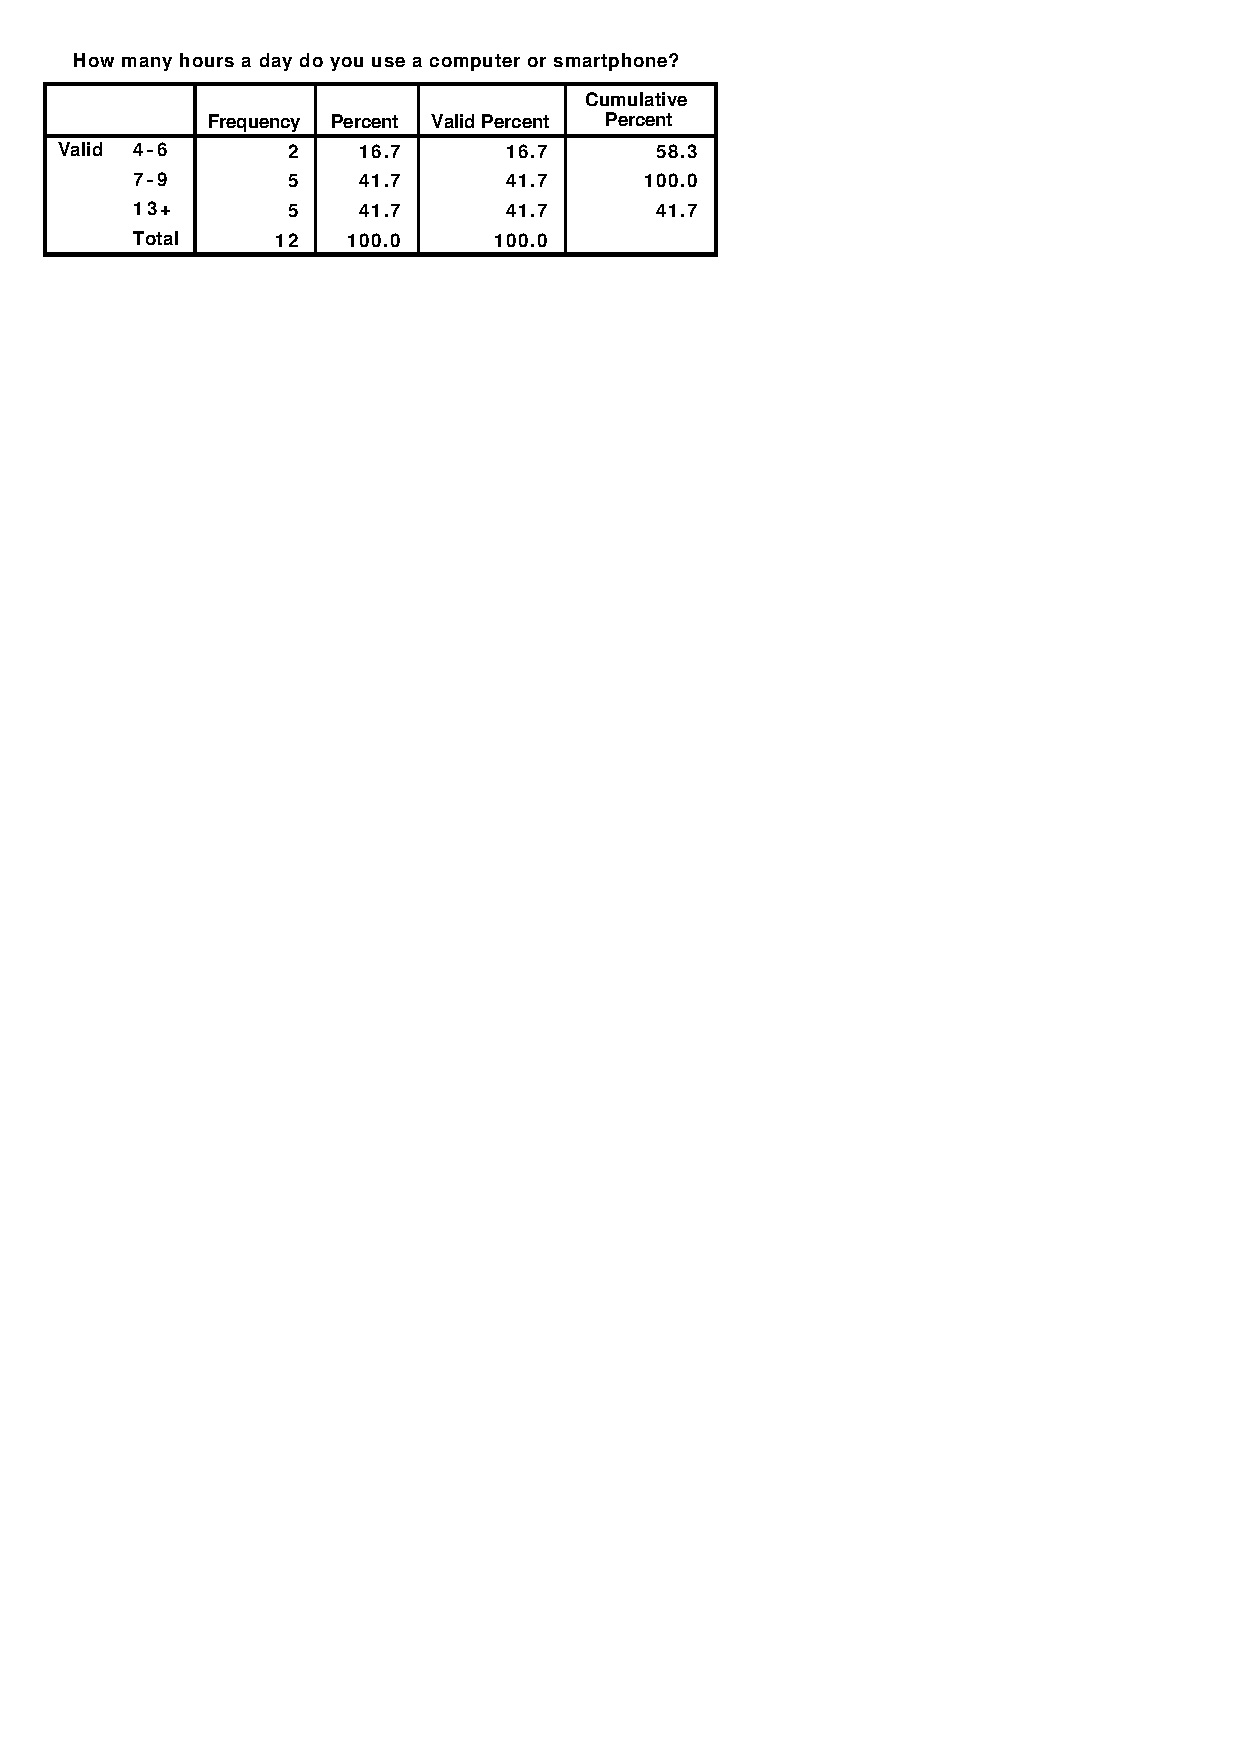
\includegraphics{figures/ComputerHours.pdf}}
\caption{Device usage by participant}
\label{fig:partic_computerHours}
\end{figure}

\begin{figure}[ht]
\centerline{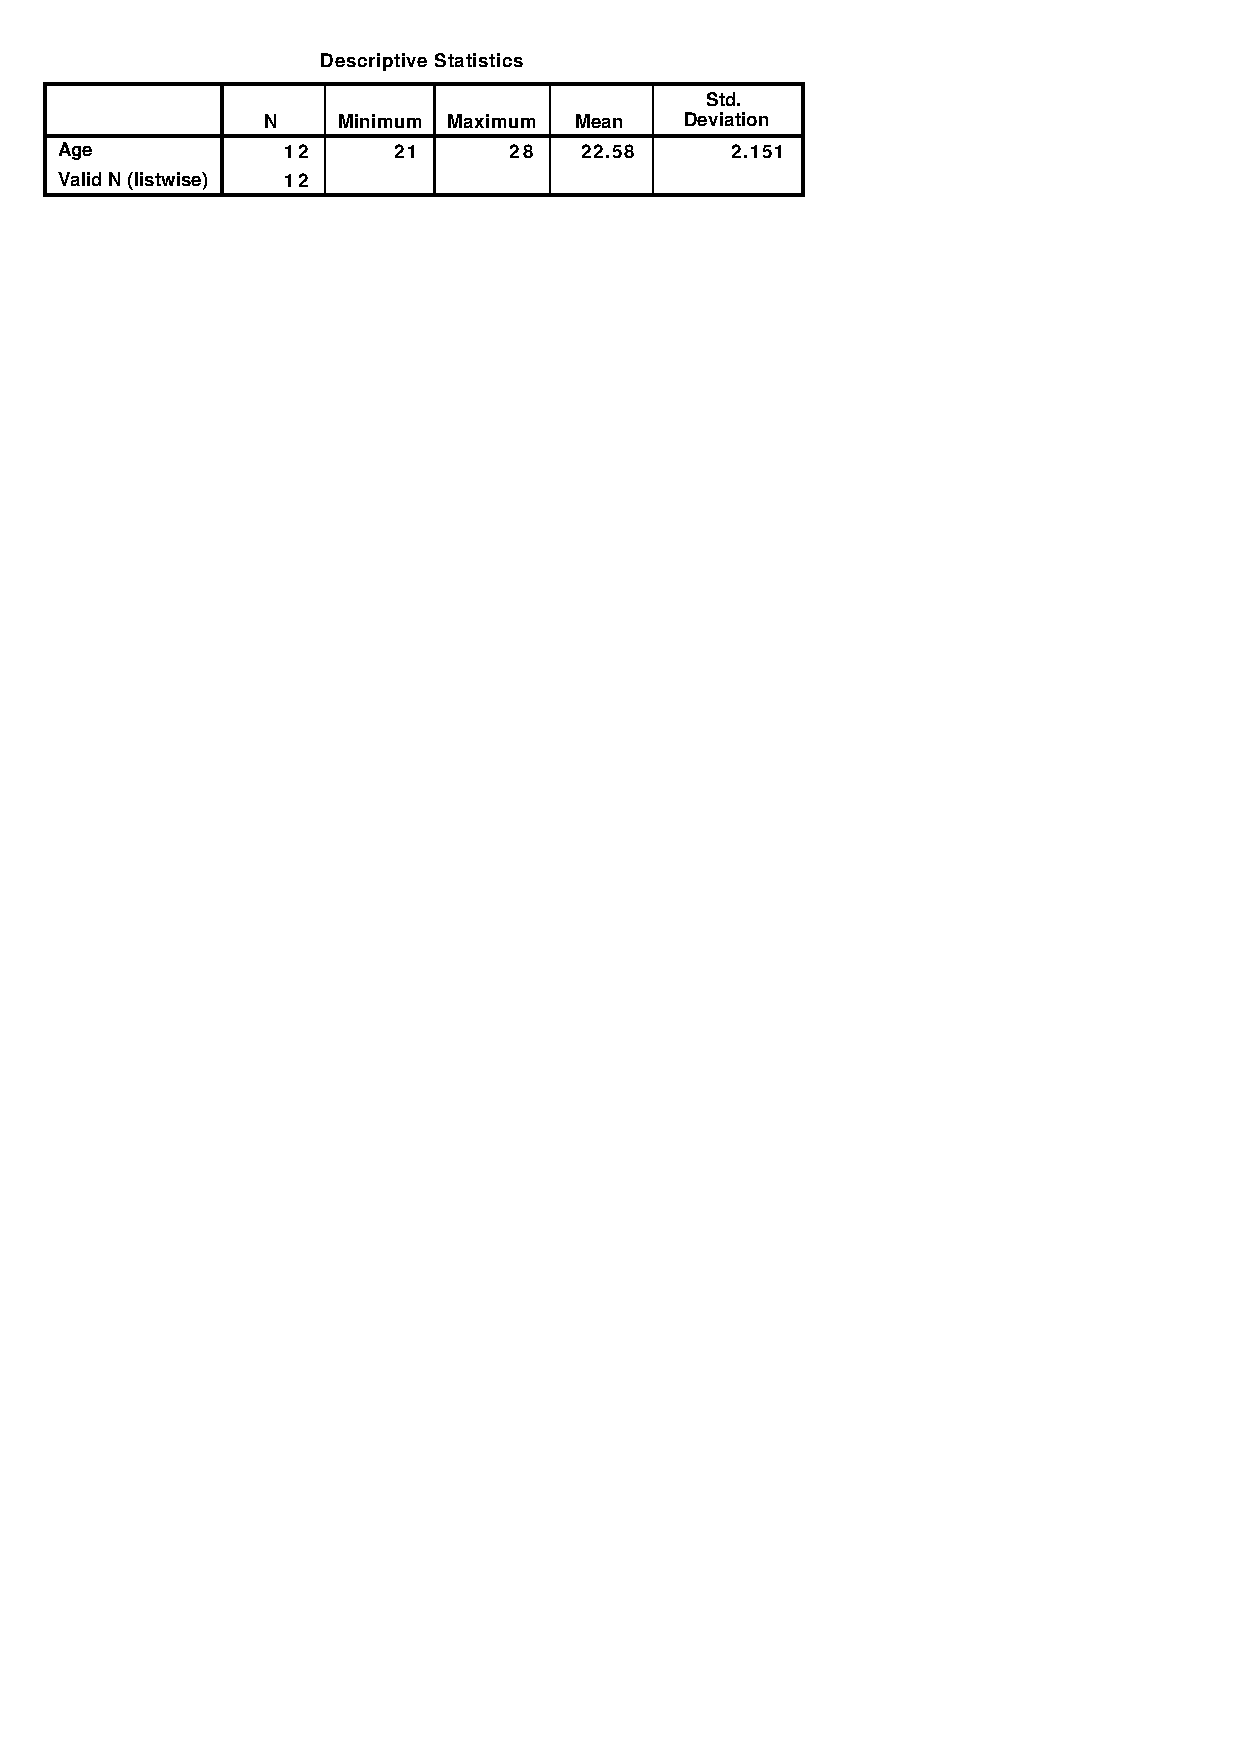
\includegraphics{figures/Age.pdf}}
\caption{Age of participant}
\label{fig:partic_age}
\end{figure}

\begin{figure}[ht]
\centerline{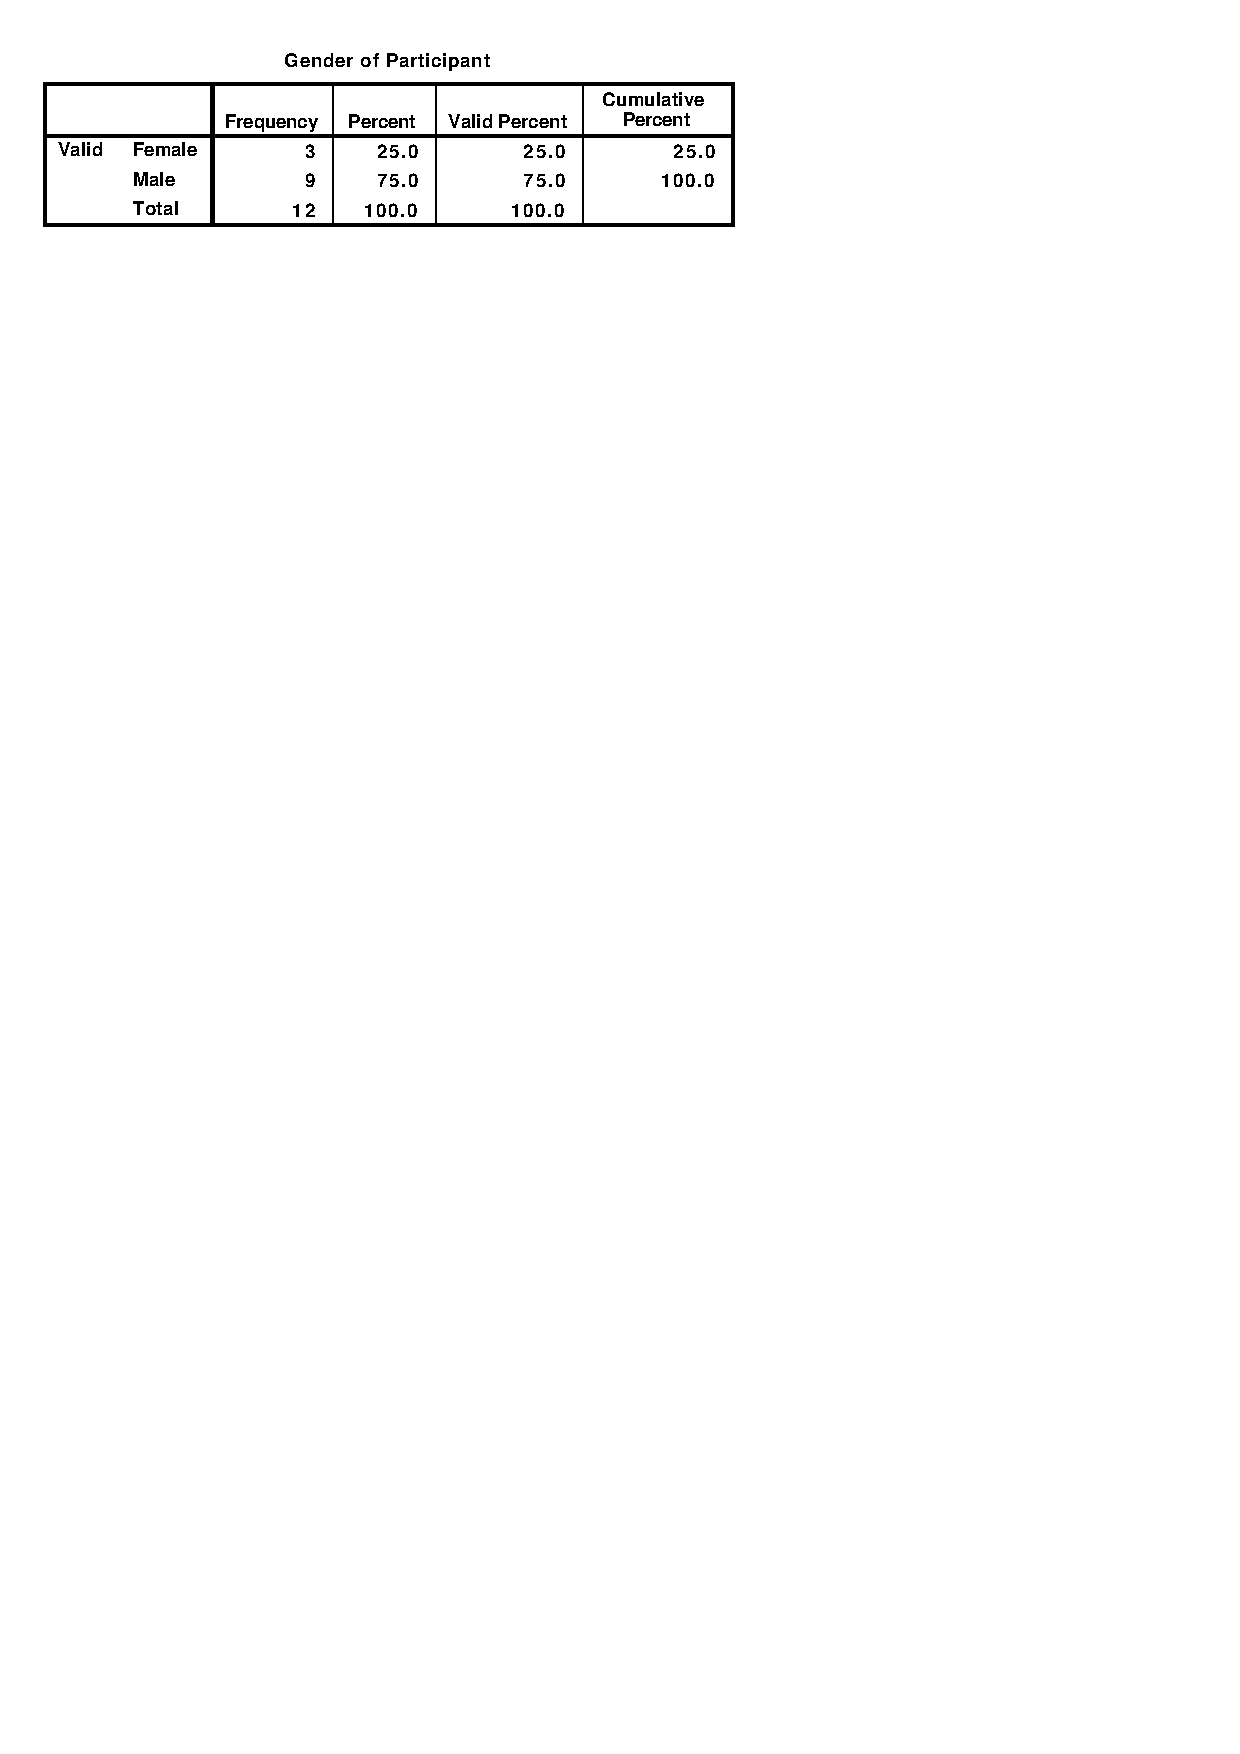
\includegraphics{figures/Gender.pdf}}
\caption{Gender of participant}
\label{fig:partic_gender}
\end{figure}

\begin{figure}[ht]
\centerline{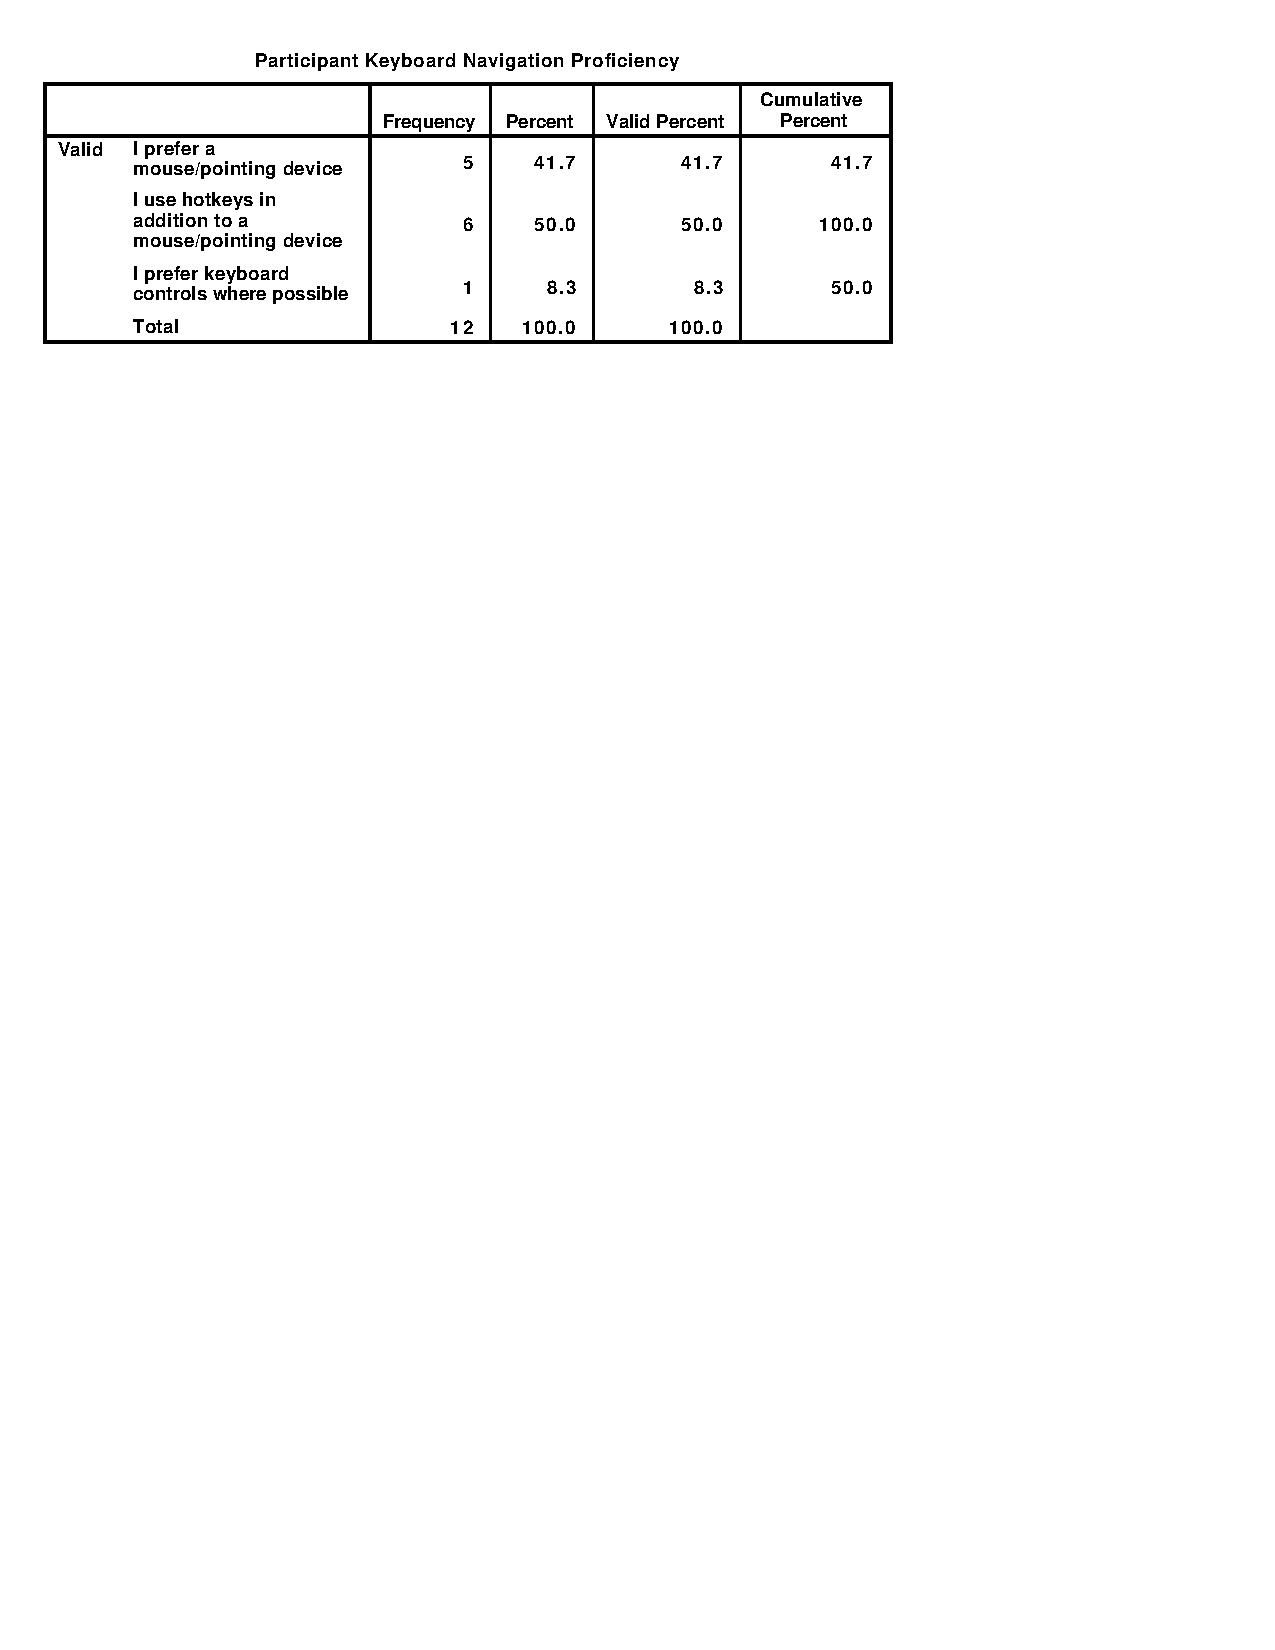
\includegraphics{figures/Proficiency.pdf}}
\caption{Keyboard Navigation Proficiency of Participants}
\label{fig:partic_proficiency}
\medskip
\small
Participants were asked to pick which of these sentiments they identified best with. The statements attempted to describe a proficiency scale for keyboard usage:
\begin{enumerate}
\item I need a mouse/pointing device
\item I prefer a mouse/pointing device
\item I use hotkeys in addition to a mouse/pointing device
\item I prefer keyboard controls where possible
\item I strongly prefer full keyboard support
\end{enumerate}
Votes were cast only for the middle descriptors, 2--4.
\end{figure}

\begin{figure}[ht]
\centerline{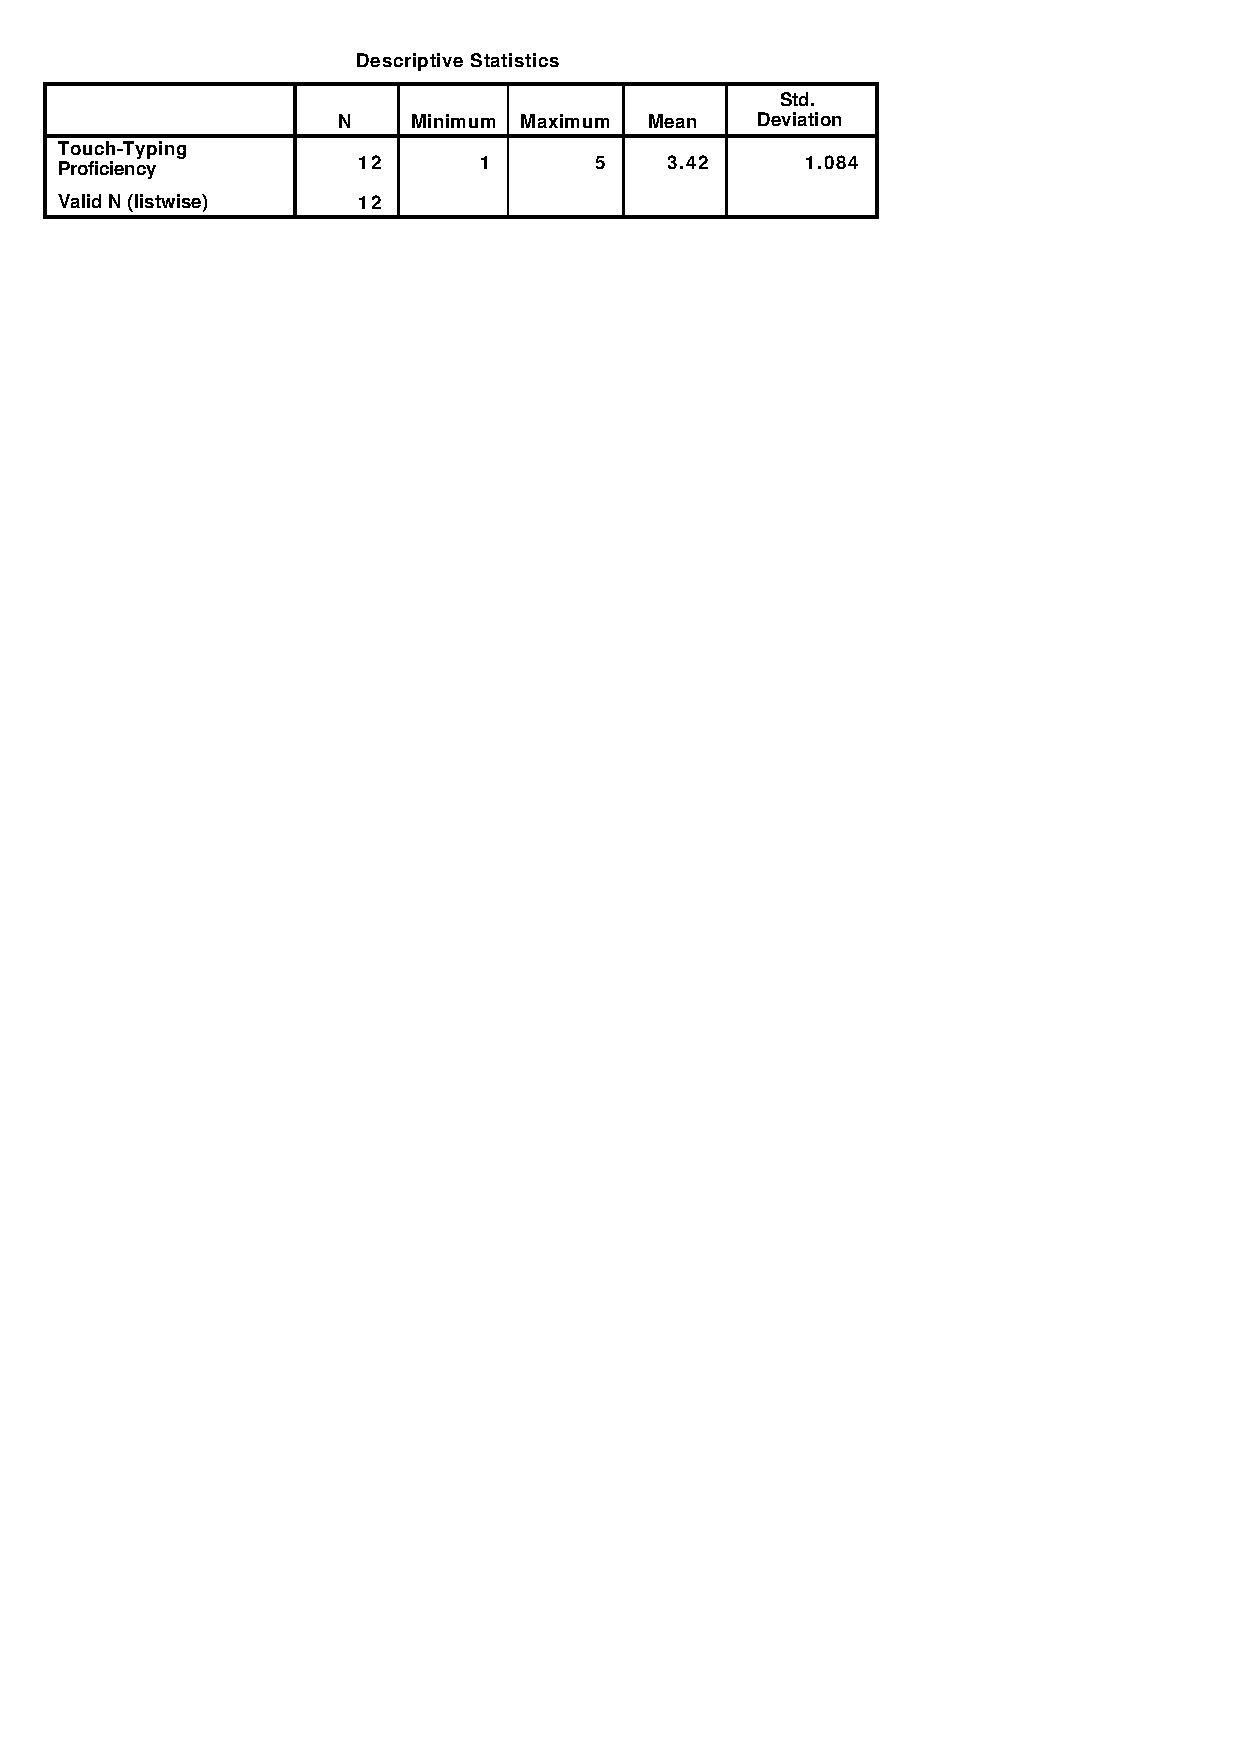
\includegraphics{figures/TouchTyping.pdf}}
\caption{Touch-Typing Proficiency of Participants}
\label{fig:partic_ttype}
\medskip
\small
Touch-typing proficiency was rated on a five-point scale ranging from the sentiment `I look at every key before pressing' to `I always type without even a reference glance at the keyboard'.
\end{figure}


\pagebreak
\printglossary[title=Terms]

%\nocite{*}
%\nocite{Doe:2009:Online}
\pagebreak
\printbibliography

\pagebreak
\chapter{Appendices}

\begin{figure}[ht]
	\begin{enumerate}
		\item \url{https://www.halifax-online.co.uk/personal/logon/login.jsp}
		\item \url{https://www.kickstarter.com/signup?ref=nav}
		\item \url{http://www.bbc.co.uk/}
		\item \url{http://www.bath.ac.uk/library/subjects/comp-sci/}
		\item \url{http://www.youtube.com/}
		\item \url{http://www.amazon.co.uk/s/ref=nb_sb_noss_2?url=search-alias%3Daps&field-keywords=pillow&rh=i%3Aaps%2Ck%3Apillow}
		\item \url{http://www.megatokyo.com/}
		\item \url{http://en.wikipedia.org/wiki/Computer}
	\end{enumerate}
	\caption{URLs used in tasks (full study)}
	\label{fig:fullStudyURLs}
	\medskip
	\small
\end{figure}

\end{document}